\documentclass[12pt]{article}
\usepackage[a4paper, margin=1in]{geometry}
\usepackage{titlesec}
\usepackage{graphicx}
\usepackage{fancyhdr}
\usepackage{hyperref}
\usepackage{longtable}
\usepackage{enumitem}
\usepackage{color}
\usepackage{array}
\usepackage{setspace}
\usepackage{caption}
\usepackage{subcaption}

\setlength{\parskip}{0.5em}
\setlength{\parindent}{2em}
\pagestyle{fancy}
\fancyhf{}
\rhead{CPT304 Assignment 2}
\lhead{Open Source Contribution}
\rfoot{Page \thepage}

% Title formatting
\titleformat{\section}{\Large\bfseries}{\thesection}{1em}{}
\titleformat{\subsection}{\normalsize\bfseries}{\thesubsection}{1em}{}

\begin{document}

% -------------------
% Title Page Content
% -------------------
\noindent
\textbf{\Large CPT304 Assignment 2 Report} \\[0.5em]
\textbf{Title:} Open-Source Investigation and Contribution \\[0.5em]
\textbf{Group Members:} 
\\ [0.5em]
\textbf{Date:} \today

\vspace{1em}
\hrule
\vspace{1.5em}

% -------------------
% Abstract
% -------------------
\section*{Abstract}
The open-source ecosystem is the innovation driver of modern software engineering, and learning about open-source values and practices is of great significance to developers. This course report presents our team's analysis of the entire process from contributors' workflows to the acceptance of contributions, with actual contributions made in the open-source project \texttt{Python-Scripts}. 

We first investigated the meaning and value of open source, elaborating on different types of open-source licenses, followed by an analysis of governance models and contribution processes within the open-source community. Based on this research, we explored real-world open-source processes through practice. In our contribution plan, all four team members collaborated by enhancing code and documentation for the open-source project while dividing tasks related to this report's content. 

We submitted a pull request to the \texttt{Python-Scripts} repository, contributing beginner-friendly Python scripts with practical functionality and improving the project’s documentation. Our contributions are currently under review by the maintainers. Through this process, we demonstrated effective teamwork and gained valuable experience in open-source collaboration.

% -------------------
% 1. Introduction
% -------------------
\section{Introduction}
Open source software is a pillar of modern engineering practice, providing publicly auditable codebases and an active peer review process. Contributing to the open source community allows developers to gain practical experience in version control, issue categorization, continuous integration, and distributed collaboration. In this report, our team selected the \texttt{Python-Scripts} project. 

\texttt{Python-Scripts} is a community-maintained repository that brings together over 60 independent Python tools, each located in its own folder with explanatory README files. The project uses the MIT license, has over 700 GitHub stars, and is tagged with labels suitable for beginners (such as "good-first-issue"). 

We chose it for three reasons: 
\begin{itemize}
    \item \textbf{Technical scope fit:} The repository covers file input/output, web automation, and simple machine learning demonstrations—technologies we have encountered in our course.
    \item \textbf{Low entry barrier:} The modular folder structure allows newcomers to add or optimize individual scripts without deep coupling with the rest of the codebase.
    \item \textbf{Responsive maintainers:} Historical PR data shows shorter review cycles which significantly increases the likelihood of our contributions being merged and available for evaluation verification.
\end{itemize}


% -------------------------------
% 2. Open Source Investigation
% -------------------------------
\section{Open Source Investigation}

\subsection{Understanding the Open Source Community}
We studied the philosophy behind open source: transparency, collaboration, and community. The core of the open-source movement lies in the principle of "sharing is progress." When source code is made publicly available, anyone can read, improve, and redistribute it, which promotes a highly transparent collaborative culture on a global scale. 

Developers are no longer isolated islands but aggregate into efficient communities through mailing lists, Issues discussion areas, and instant messaging tools. For newcomers, the most direct benefit is the quick acquisition of mature code and learning best practices; for enterprises, open-source means lower cost of trial and error and higher speed of innovation; for us students, we can learn coding standards in actual production, and make connections with peers, receive code reviews, and learn best practices through the open-source community. 

The open-source community usually follows a governance model of consensus-driven and gatekeeping by maintainers: the majority opinion guides the technical direction, but the power to merge code ultimately rests with a few core maintainers.

\subsection{Open Source Licenses}
The key licenses we investigated include:

\begin{itemize}
    \item \textbf{MIT License}: Highly permissive, allows reuse with attribution.
    \item \textbf{GPL v3}: Requires derivative works to remain open.
    \item \textbf{Apache 2.0}: Includes explicit patent grants.
\end{itemize}
    The following is a detailed introduction to the licenses we researched.
    
    \noindent\textbf{MIT License}

    The MIT License is one of the simplest and most permissive open-source licenses currently available. It allows anyone to use, copy, modify, and publish code with almost no restrictions, including commercializing it. Developers only need to retain the original copyright notice and license text when distributing the source code to use it legally. The license explicitly states that the software is provided "as is," without any form of warranty liability. The author assumes no responsibility for issues related to functionality, security, or suitability. This provides developers with great flexibility while reducing legal risks. However, the MIT License does not cover patent rights nor does it provide guidance on trademark usage. Therefore, compliance should be assessed when the code involves significant algorithms or trademark usage. Due to its high compatibility, this license is widely used in front-end frameworks (such as React and Vue) as well as various scaffolding tools and lightweight general-purpose libraries.

    \noindent\textbf{GNU General Public License v3 (GPL v3)}

    GPL v3 is a strong Copyleft open-source license released by the Free Software Foundation in 2007. The agreement requires that any derivative works built on GPL v3 code must be made available under the same license whenever they are distributed, ensuring that software freedom can be inherited and continued. In addition to inheritance requirements, GPL v3 also prohibits preventing users from freely using or modifying the software through DRM technologies or hardware restrictions. Furthermore, the agreement includes an automatic patent grant clause, whereby contributors automatically grant their patent licenses related to their code to users. Moreover, if a user who uses GPL v3 licensed code initiates a patent lawsuit against the author, their originally granted patent rights will also be immediately terminated. This agreement is widely used in free software projects such as the GNU toolchain, GDB, Bash, and other core components of operating systems and is a representative license advocating for software freedom.


  \noindent\textbf{Apache License 2.0}

    The Apache License 2.0, released by the Apache Software Foundation, is a permissive yet more mature open-source license. It allows users to freely use, modify, and distribute code while further adding provisions for patent rights protection, making it widely adopted in enterprise-level projects. The license explicitly states that contributors automatically grant users a global, irrevocable, royalty-free patent license related to their contributions. Additionally, it introduces a patent retaliation termination mechanism: if a user initiates a patent lawsuit against the original author due to the use of this code, their licensing rights will be immediately revoked. To ensure compliance, Apache 2.0 requires that LICENSE and NOTICE files be retained during distribution to document changes and third-party components relied upon. This plays an important role in corporate governance and compliance audits. Apache 2.0 is compatible with GPL v3 but not with GPL v2 and is currently the mainstream choice in cloud computing and machine learning fields. Notable open-source projects such as Hadoop, Kafka, Spark, TensorFlow all utilize this license.
% \vspace{1em}
\noindent\textbf{Comparison}

The \textbf{MIT License} is highly permissive and ideal for developers aiming to promote projects quickly, encourage contributions, or allow commercial closed-source use. It is widely adopted in front-end frameworks, development tools, and lightweight libraries.

The \textbf{Apache 2.0 License} retains MIT’s flexibility while adding patent protection and anti-suit clauses, making it well-suited for enterprise use. It is commonly used in cloud computing, distributed systems, middleware, and machine learning frameworks.

The \textbf{GPL v3 License} requires all derivative works to remain open source, making it suitable for educational, toolchain, and public-interest projects. Developers who prioritize software freedom and want to prevent proprietary reuse often choose GPL v3.


\subsection{Ways to Contribute}

Common ways to contribute to open source can be roughly divided into four categories: 

1. \textbf{Code Contributions}. If you have made changes to the repository code, you can add features, fix bugs, or optimize performance by submitting a Pull Request (PR). This is the most direct technical contribution and needs to follow the project's coding standards and contribution process.

2. \textbf{Documentation Improvement}. You can write or improve usage instructions for the repository code, and you can also add API documentation, quick start guides, code comments, etc., to enhance the project's readability and maintainability. This type of contribution is suitable for beginners.

3. \textbf{Issue Reporting \& Triage} You can submit bug reports, feature suggestions in the community's issues, or participate in discussions of existing issues to assist maintainers in identifying problems, categorizing priorities, and supplementing reproduction steps.

4. \textbf{Testing \& Code Review}. You can follow the principles of software testing to write reasonable and reliable test code, helping to verify whether new features in the repository are functioning correctly, how compatibility is across different environments, and assessing performance. You can also participate in reviewing others' PRs, providing suggestions for modifications or confirming the logical soundness.

\subsection{Finding Suitable Projects}
When filtering the open source repositories we wanted to contribute to, we first used GitHub's advanced search and set the following filter criteria: 1) Tags include "good first issue" and "help wanted" to confirm that the repository maintainers are friendly to newcomers; 2) The language is limited to Python, which aligns with our recently learned and used tech stack; 3) There has been at least one merged PR in the last month, proving that the project is active and maintainers merge contributions in a timely manner. 

Subsequently, we referred to the beginner index provided by firstcontributions.github.io for secondary filtering of search results, focusing on license types, code coupling degree, and community feedback speed. After comprehensive comparison, the \href{https://github.com/DhanushNehru/Python-Scripts}{\texttt{Python-Scripts}} repository best meets our needs. 

The \texttt{Python-Scripts} is an open-source project based on the MIT license that maintains a series of Python tool scripts. Each script in the repository is independent and easy for incremental submissions; the Issues section remains active, with maintainers publicly encouraging contributions on social media and committing to quickly merging high-quality PRs. Based on these objective indicators and their fit with learning outcomes, we ultimately identified this repository as our team's contribution target.


\subsection{Typical Contribution Process}
To effectively participate in open source projects, individual contributors typically need to go through two stages: preparation and execution. 

In the preparation stage, contributors should first have basic Git operation skills, understand the language and framework used by the project, and carefully read the project's README.md, CONTRIBUTING.md, and other related files to ensure compliance with standards and codes of conduct. 

In the execution stage, the contribution process usually includes the following steps: first, \textbf{fork} the target project repository to your own account and clone it locally for development; then implement features or fix issues on a \textbf{separate branch}. Once completed, commit and \textbf{push} your changes to the remote repository; finally, initiate a \textbf{Pull Request} via GitHub to request review and \textbf{merging} from project maintainers. 

Throughout this process, it is also important to actively respond to code review feedback and demonstrate good collaboration awareness as well as a continuous improvement attitude so that your submitted code can be positively merged.

\subsection{Contribute to \texttt{Python-Scripts}}

The \texttt{Python-Scripts} project we selected has established clear guidelines for the contribution process and community norms. Contributors must first propose suggestions to maintainers through GitHub Issues and reach a preliminary consensus before submitting changes, in order to avoid ineffective modifications and duplicate work. 

The project particularly encourages first-time participants to refer to open-source beginner resources (such as the \href{https://firstcontributions.github.io/}{First Contributions} guide) to lower the technical barrier. The specific steps for contributing to this project include: \textbf{1) Create an issue and fork the repository}; \textbf{2) Write scripts in a newly created folder along with a \texttt{README.md} documentation}; \textbf{3) Update the main repository's \texttt{README.md}, adding a brief description and link in the script list}; \textbf{4) Initiate a Pull Request referencing the corresponding issue}. 

Maintainers will decide whether to merge code after review, requiring that submissions remain concise and free of unnecessary build dependencies. Additionally, this project adheres to the general behavior guidelines of the \textit{Contributor Covenant}. 

The community encourages inclusive language, respect for diverse viewpoints, and active responses to suggestions; while harassment, discriminatory remarks, or breaches of others' privacy are strictly prohibited. Maintainers have the authority to correct inappropriate behavior, ensuring that the project's environment is open, friendly, and safe for everyone..



% ----------------------
% 3. Contribution Plan
% ----------------------
\section{Contribution Plan}

Our group has decided that the team leader will be responsible for coordinating the documentation plan and scheduling, as well as facilitating thorough discussions with all members to select an open-source project for contribution. 

Each group member will make contributions through their own local repositories after forking the selected project, and a single pull request will be submitted on behalf of the entire group. The specific division of tasks among our members is as follows.
\vspace{1em}
\begin{longtable}{|p{3cm}|p{10cm}|}
\hline
\textbf{Name} & \textbf{Task} \\
\hline
 & Coordinate scheduling; write abstracts, plans, conclusions, implementation; final layout; final contribution to \texttt{Python-Scripts} \\
\hline
 & Write license, community ecosystem, project selection; contribute to code \texttt{Python-Scripts} \\
\hline
 & Write Contribution process description, project selection, results; contribute to code \texttt{Python-Scripts} \\
\hline
 & Write contribute to \texttt{Python-Scripts}, results; submit issues to \texttt{Python-Scripts}; document and summarization; \\
\hline
\end{longtable}

% ----------------------
% 4. Implementation
% ----------------------
\section{Implementation}

We followed a collaborative workflow using GitHub. First we forked the upstream repository \texttt{Python-Scripts}.
Then we cloned the local repository and switched to the feature/video branch for development.

We have collaboratively developed a \textit{video\_contact\_sheet} feature on this branch. The \textit{video\_contact\_sheet} is a set of scripts written in pure Python that can batch-generate "contact sheets" for any video file—a grid of thumbnails composed of several keyframes, with metadata such as duration, resolution, and encoding format attached at the bottom. The script automatically detects scene changes, selects representative frames, and arranges them into an A4-sized JPEG; it can quickly process hundreds or thousands of clips using multithreading. 

The positioning of \texttt{Python-Scripts} is single-file or small directory scripts that solve everyday practical problems. The existing entries involve web scraping, PDF manipulation, and mini-games, but there is a lack of video processing tools.

This project is mainly applied in the following scenarios to address some pain points: 1) Quick screening: In content review, course editing, or monitoring playback scenarios, technicians often need to "glance" at a video to determine whether it's worth watching closely. Traditional methods either involve dragging and playing the entire segment or manually taking screenshots, which are time-consuming and labor-intensive. Contact sheets allow users to grasp the summary of materials within ten seconds. 2) Dataset quality inspection: When researching or training video-AI models, it’s often necessary to check if annotations are off-track, if resolutions are consistent, or if black frames/test cards have been mixed in. Running through the entire dataset in batches allows for easy visual identification of abnormal files. 3) Team communication: Editors, directors, and algorithm engineers often use different tools. Abstracting materials into static images shared via IM or PR significantly reduces communication costs.


% \begin{itemize}
%     \item Forked the upstream repository
%     \item Cloned and created local branches
%     \item Used VS Code, pytest, and Markdown tools for implementation
%     \item Opened pull requests with detailed descriptions and commit messages
% \end{itemize}

% ----------------------
% 5. Results
% ----------------------
%----------------------------------------
\section{Results}

The final contribution is a self-contained, modular Python utility named \textit{video\_contact\_sheet}, which generates contact sheet thumbnails for video files by extracting keyframes based on scene changes. This tool is valuable for video dataset inspection, content review, and multimedia summarization tasks.

The following is our contribution proof. Please click to access our \href{https://github.com/libran11/CPT304A2}{report repository},  \href{https://github.com/libran11/Python-Scripts}{project repository}, \href{https://github.com/DhanushNehru/Python-Scripts/issues/425}{issues}, \href{https://github.com/DhanushNehru/Python-Scripts/pull/426}{pull request}, and other information.

%--- Row 1: fork branch ---------------------------------
\begin{figure}[htbp]
  \centering
  \begin{subfigure}{0.48\textwidth}
    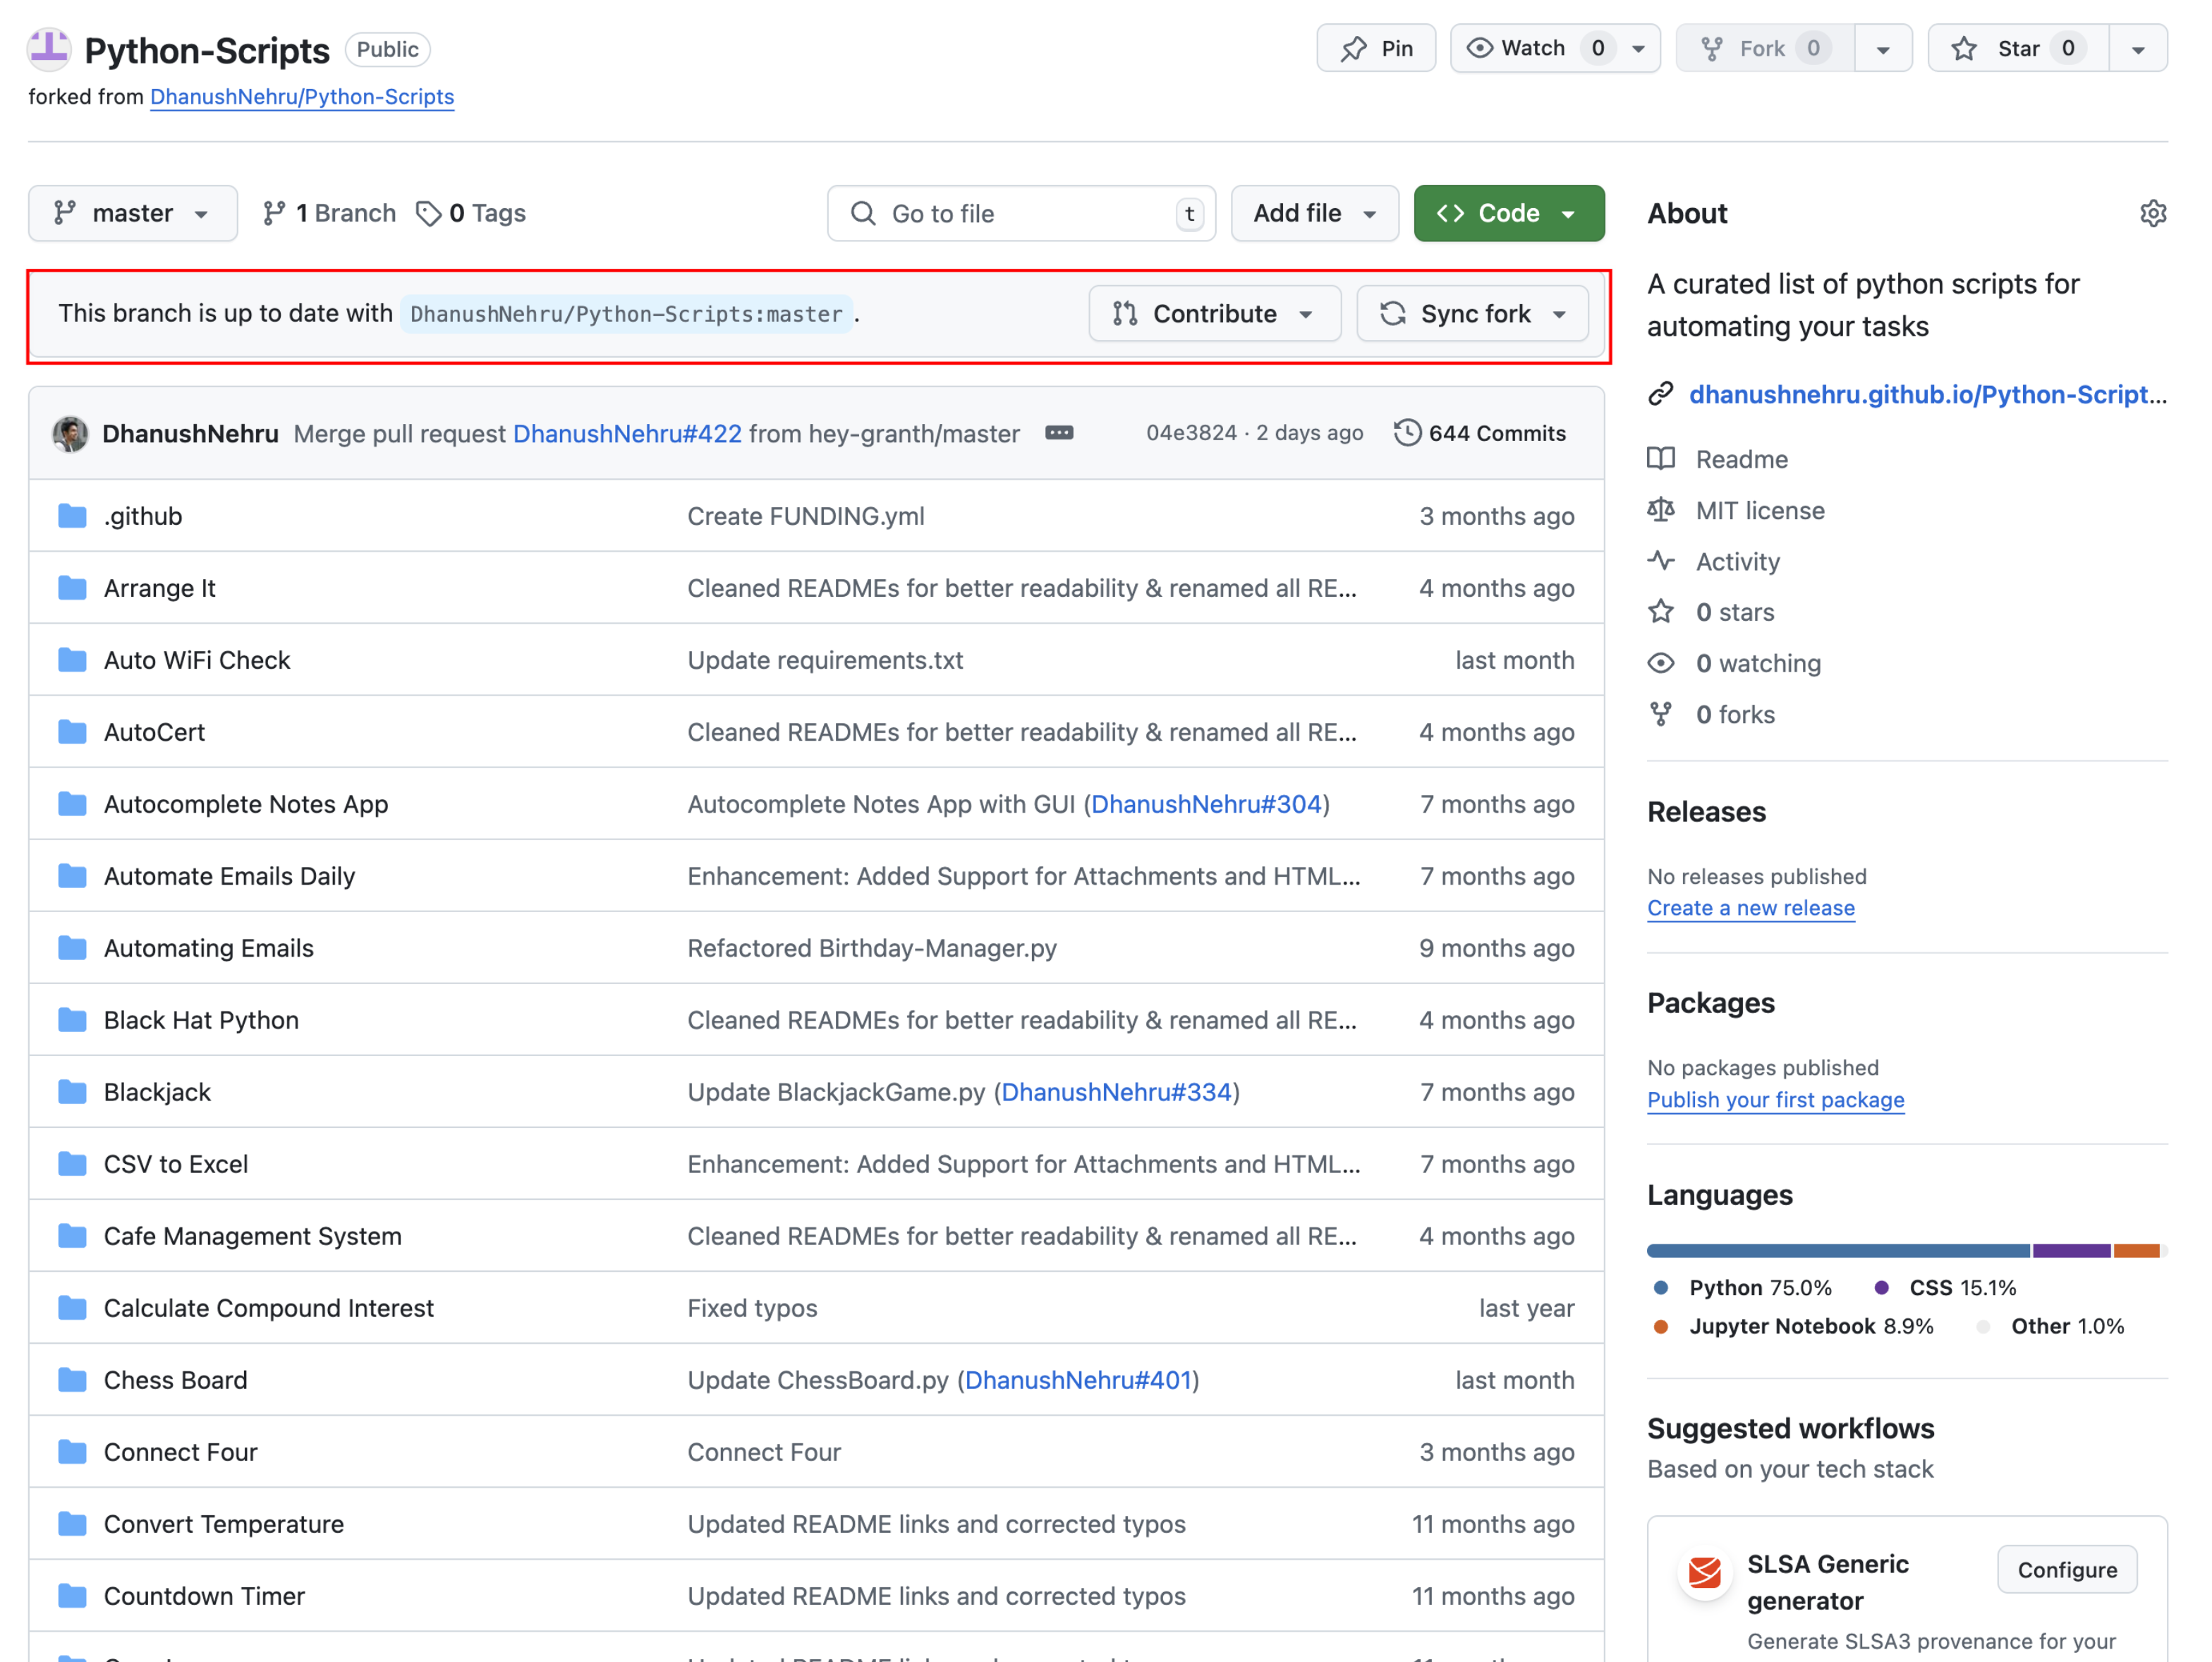
\includegraphics[width=\linewidth]{pic/fork.png}
    \caption{Forking the repository}
    \label{fig:fork}
  \end{subfigure}\hfill
  \begin{subfigure}{0.48\textwidth}
    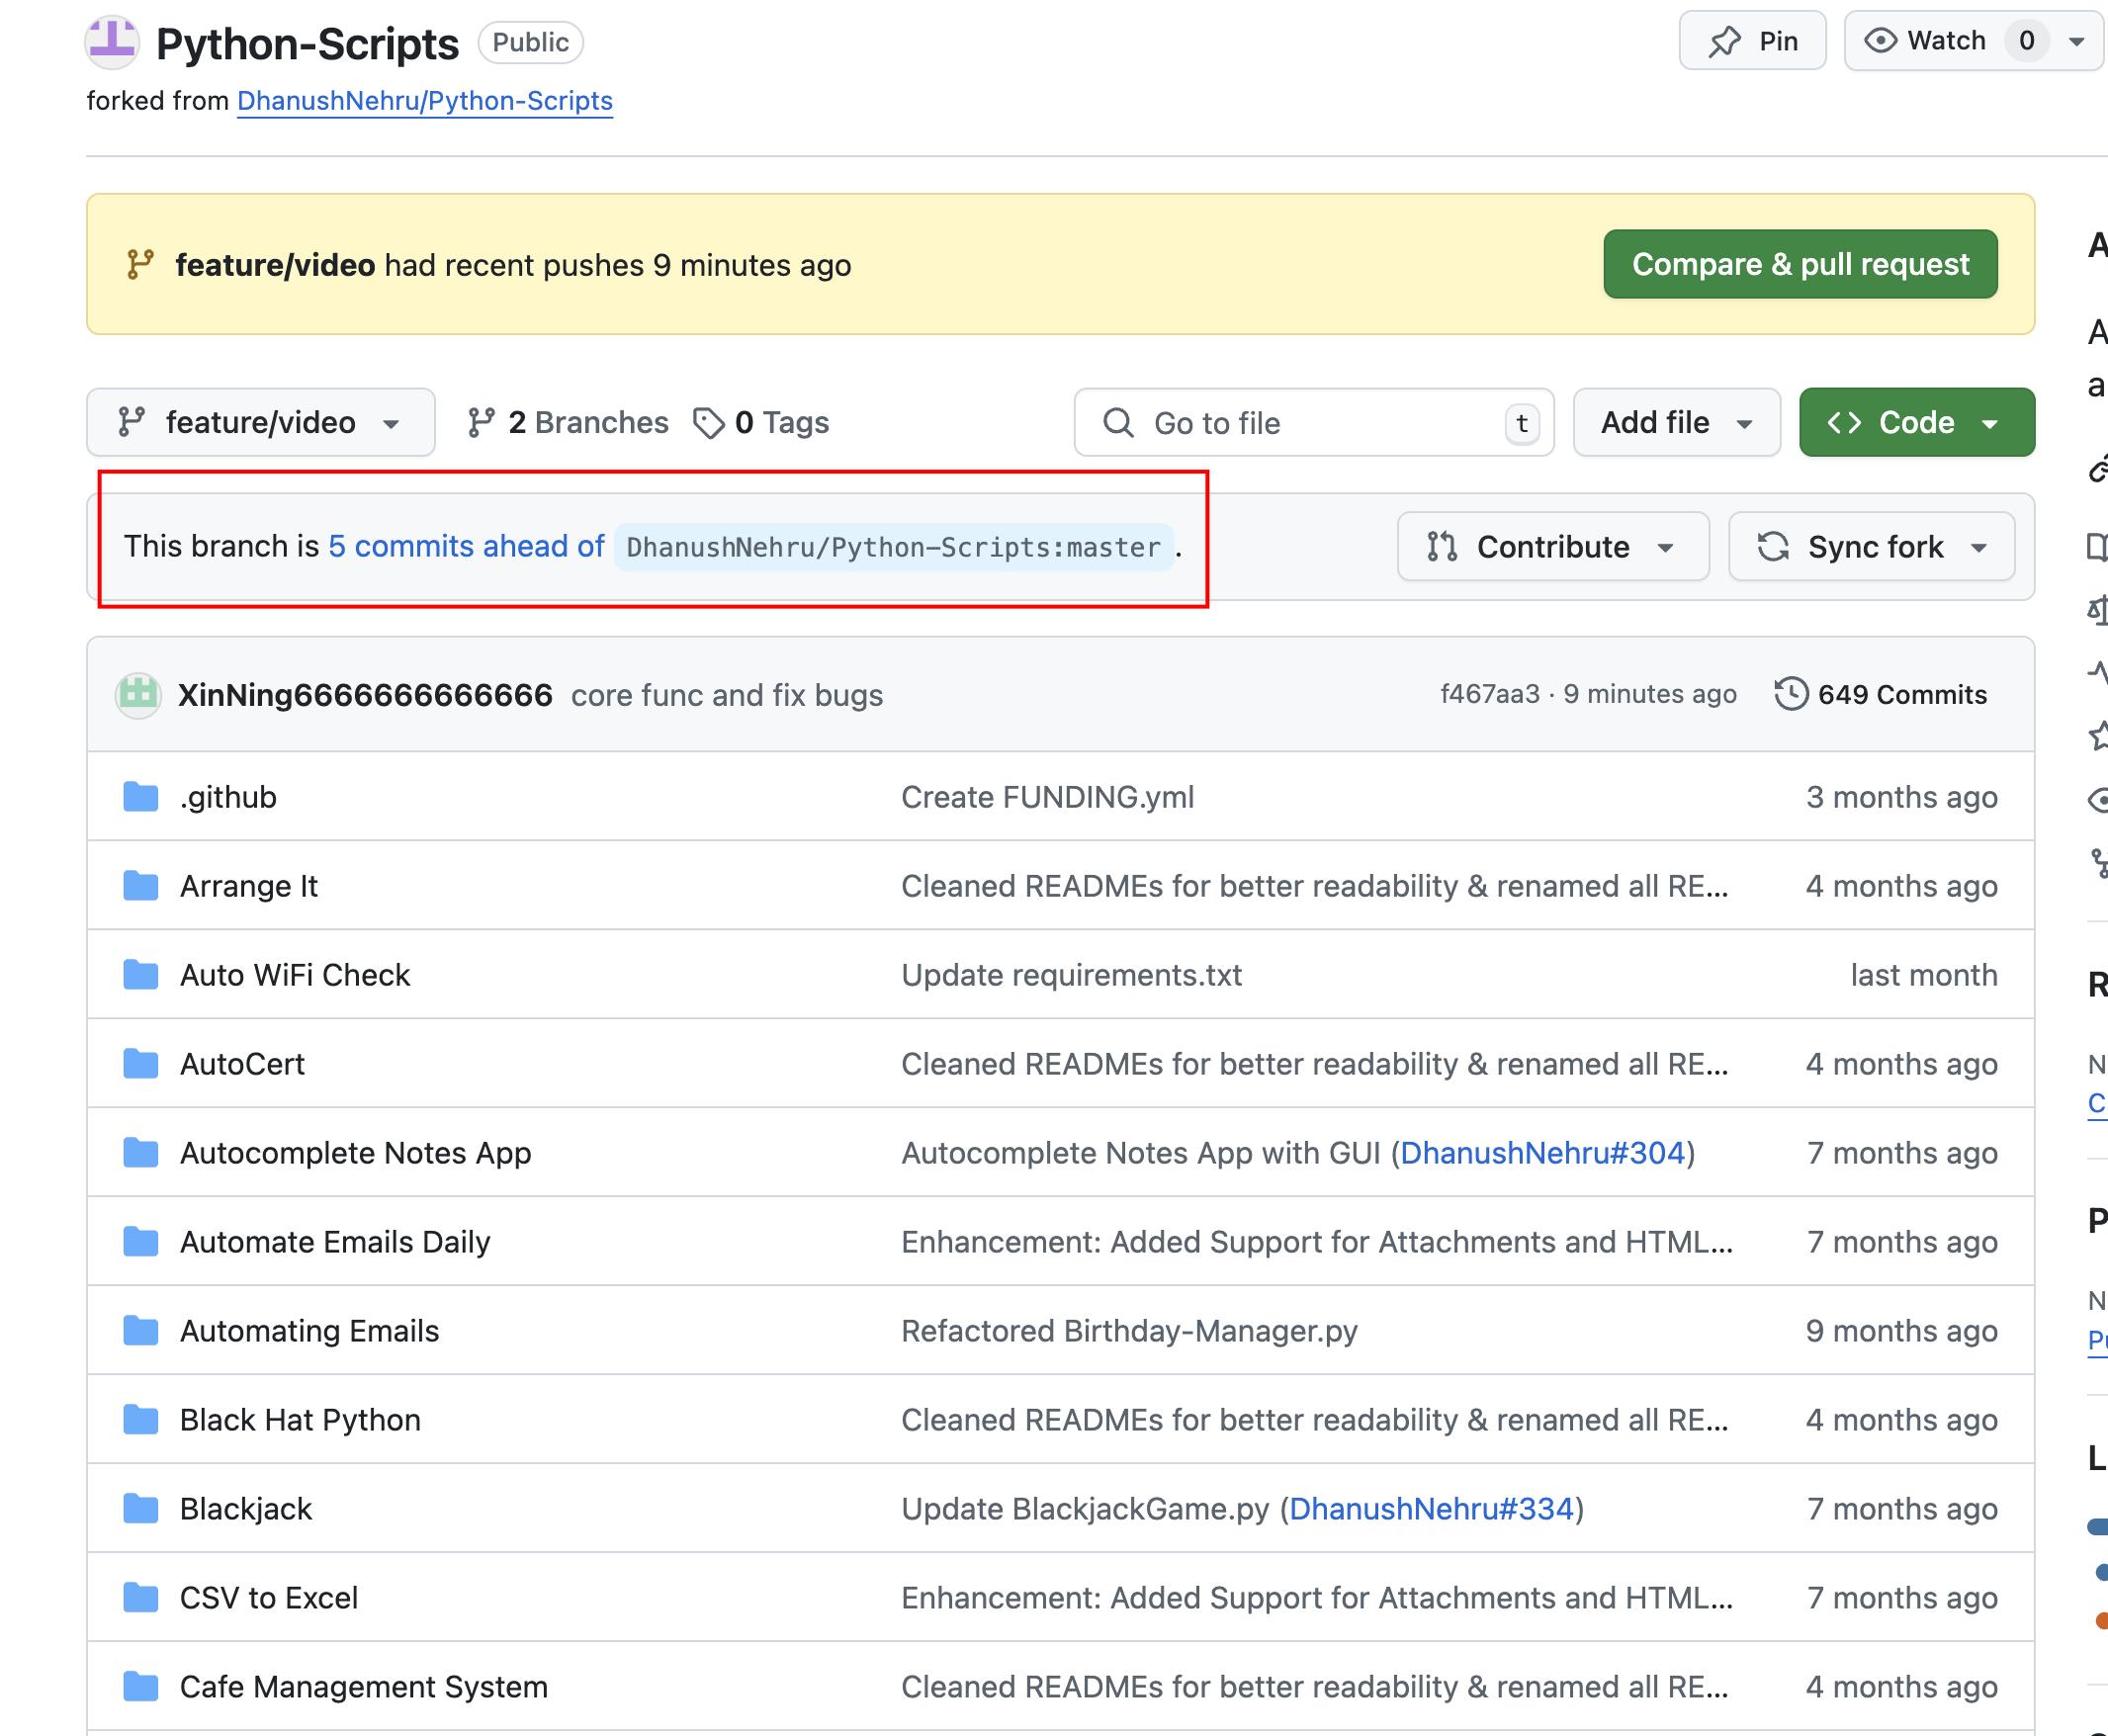
\includegraphics[width=\linewidth]{pic/branch.png}
    \caption{Creating a feature branch}
    \label{fig:branch}
  \end{subfigure}
  \caption{Repository preparation steps.}
\end{figure}

%--- Row 2: issue commit -------------------------------
\begin{figure}[htbp]
  \centering
  \begin{subfigure}{0.48\textwidth}
    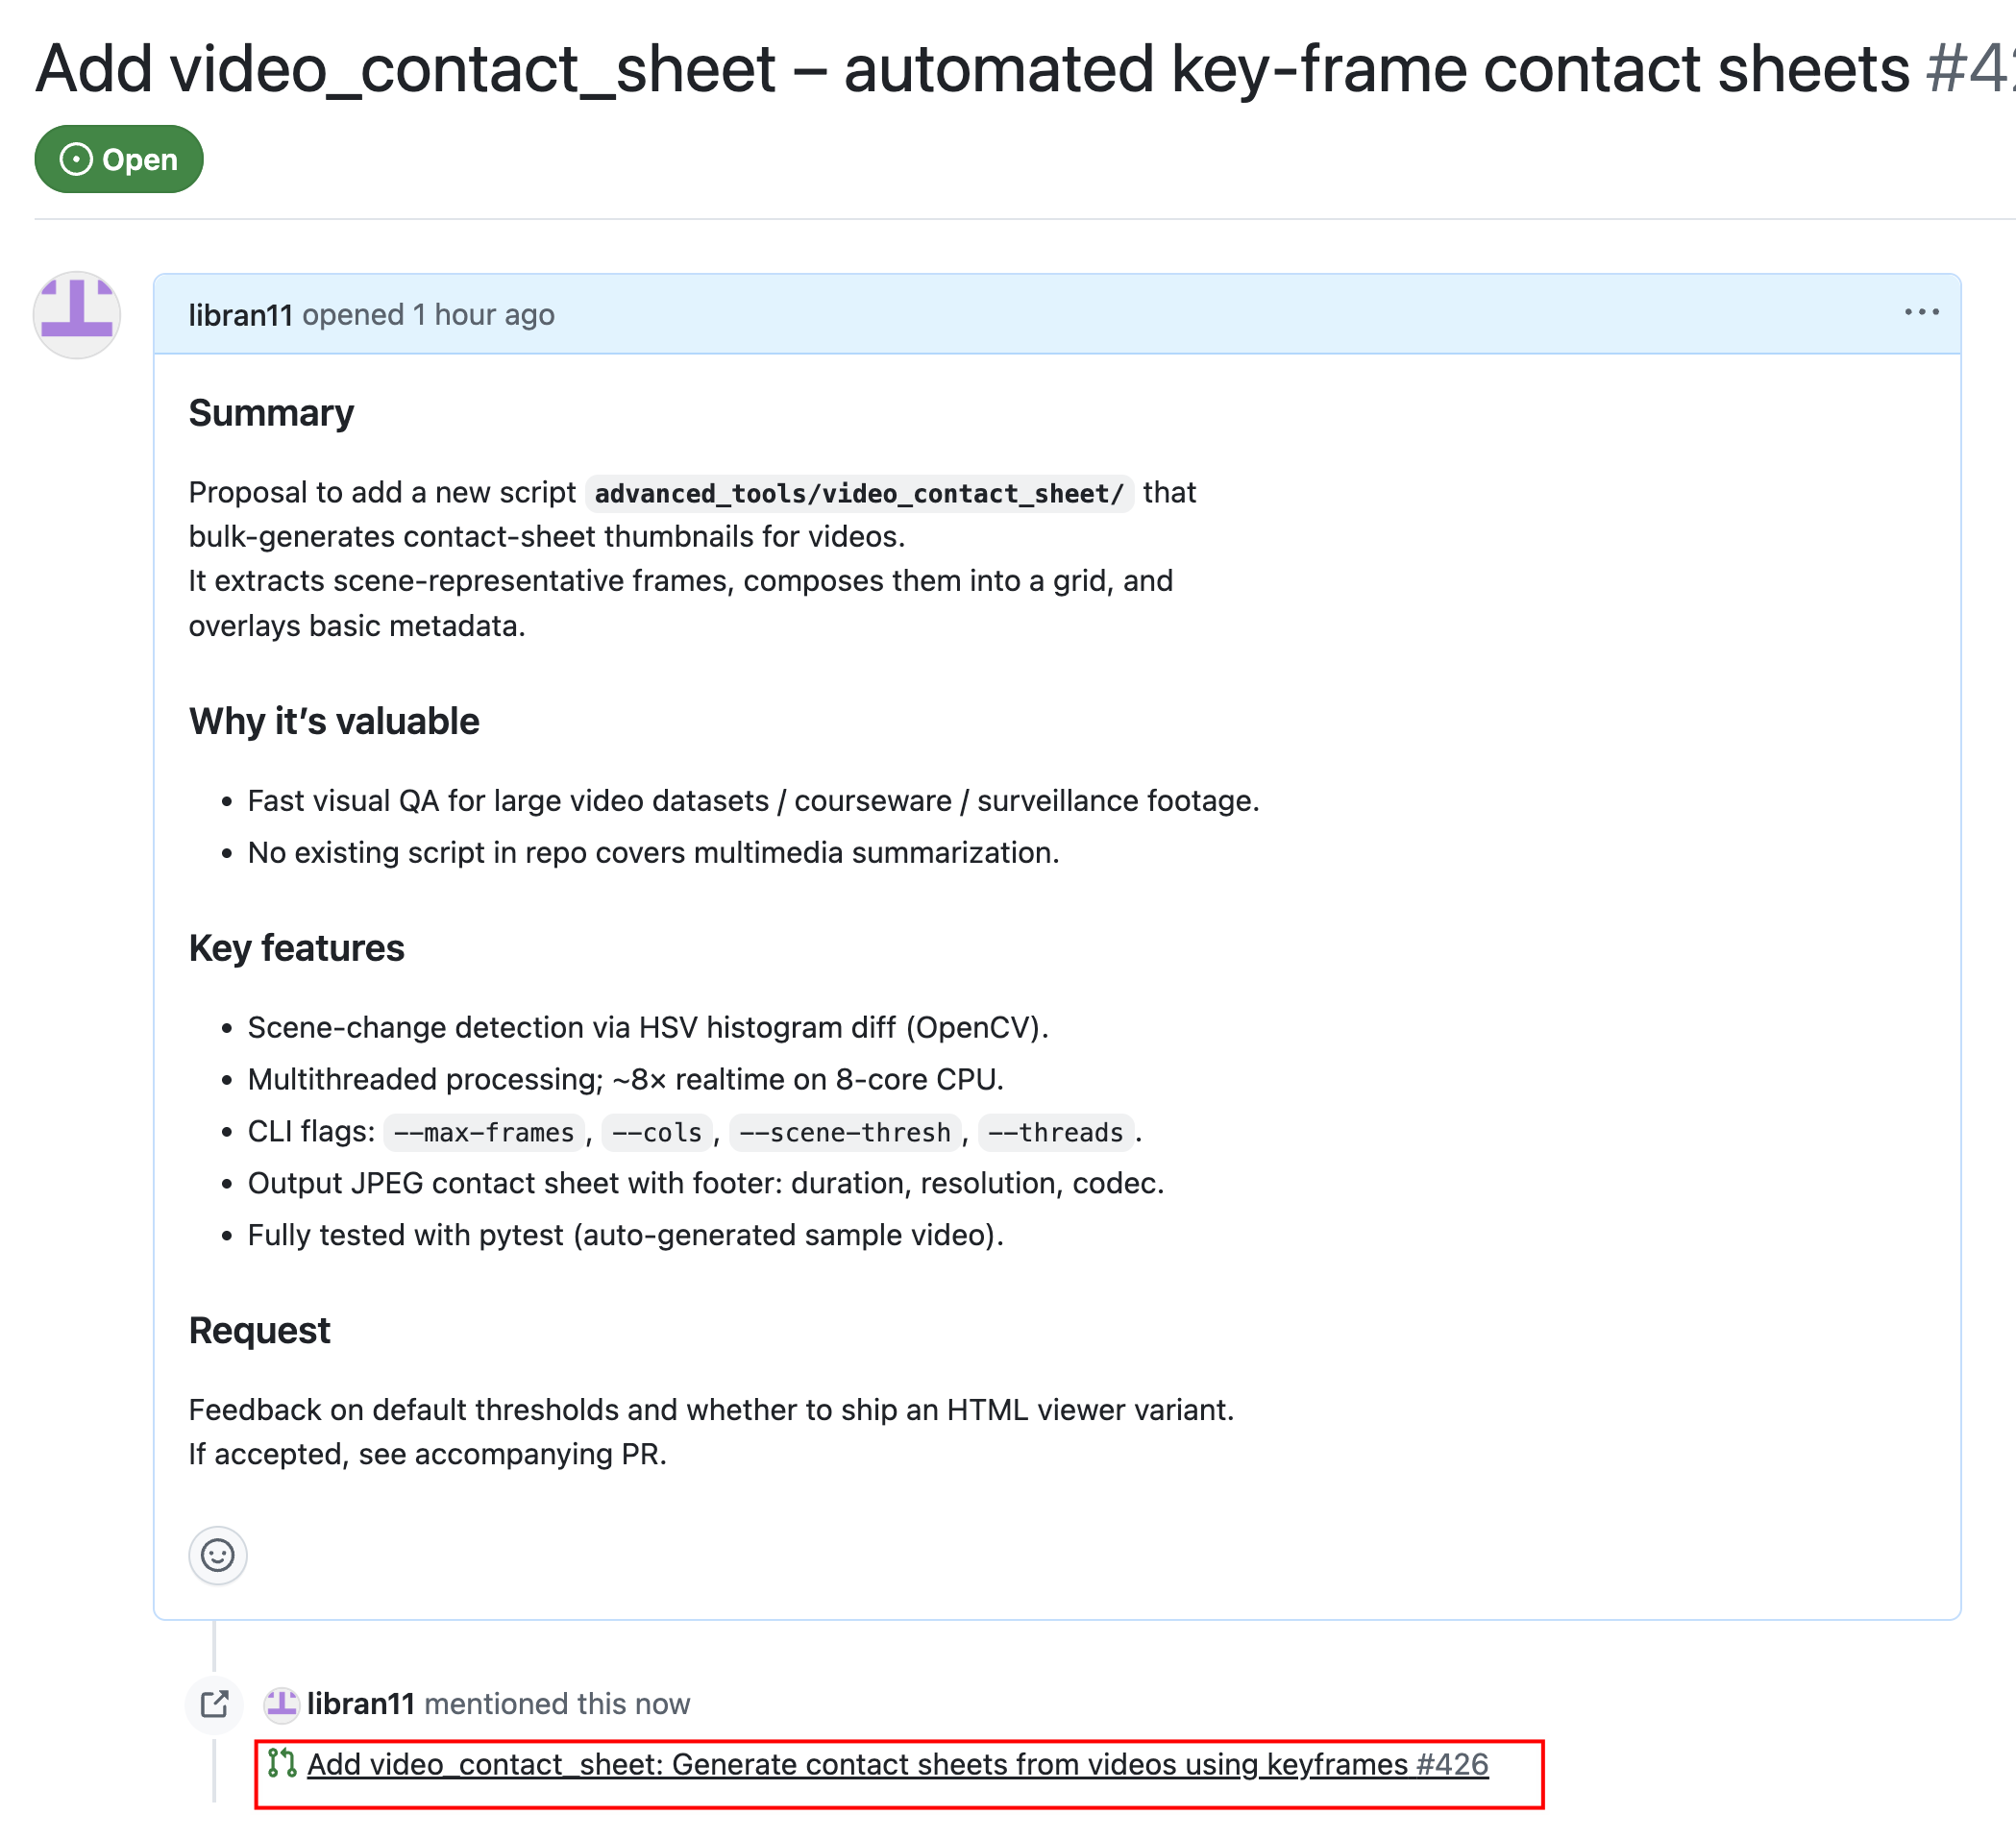
\includegraphics[width=\linewidth]{pic/issue.png}
    \caption{Opening an issue}
    \label{fig:issue}
  \end{subfigure}\hfill
  \begin{subfigure}{0.48\textwidth}
    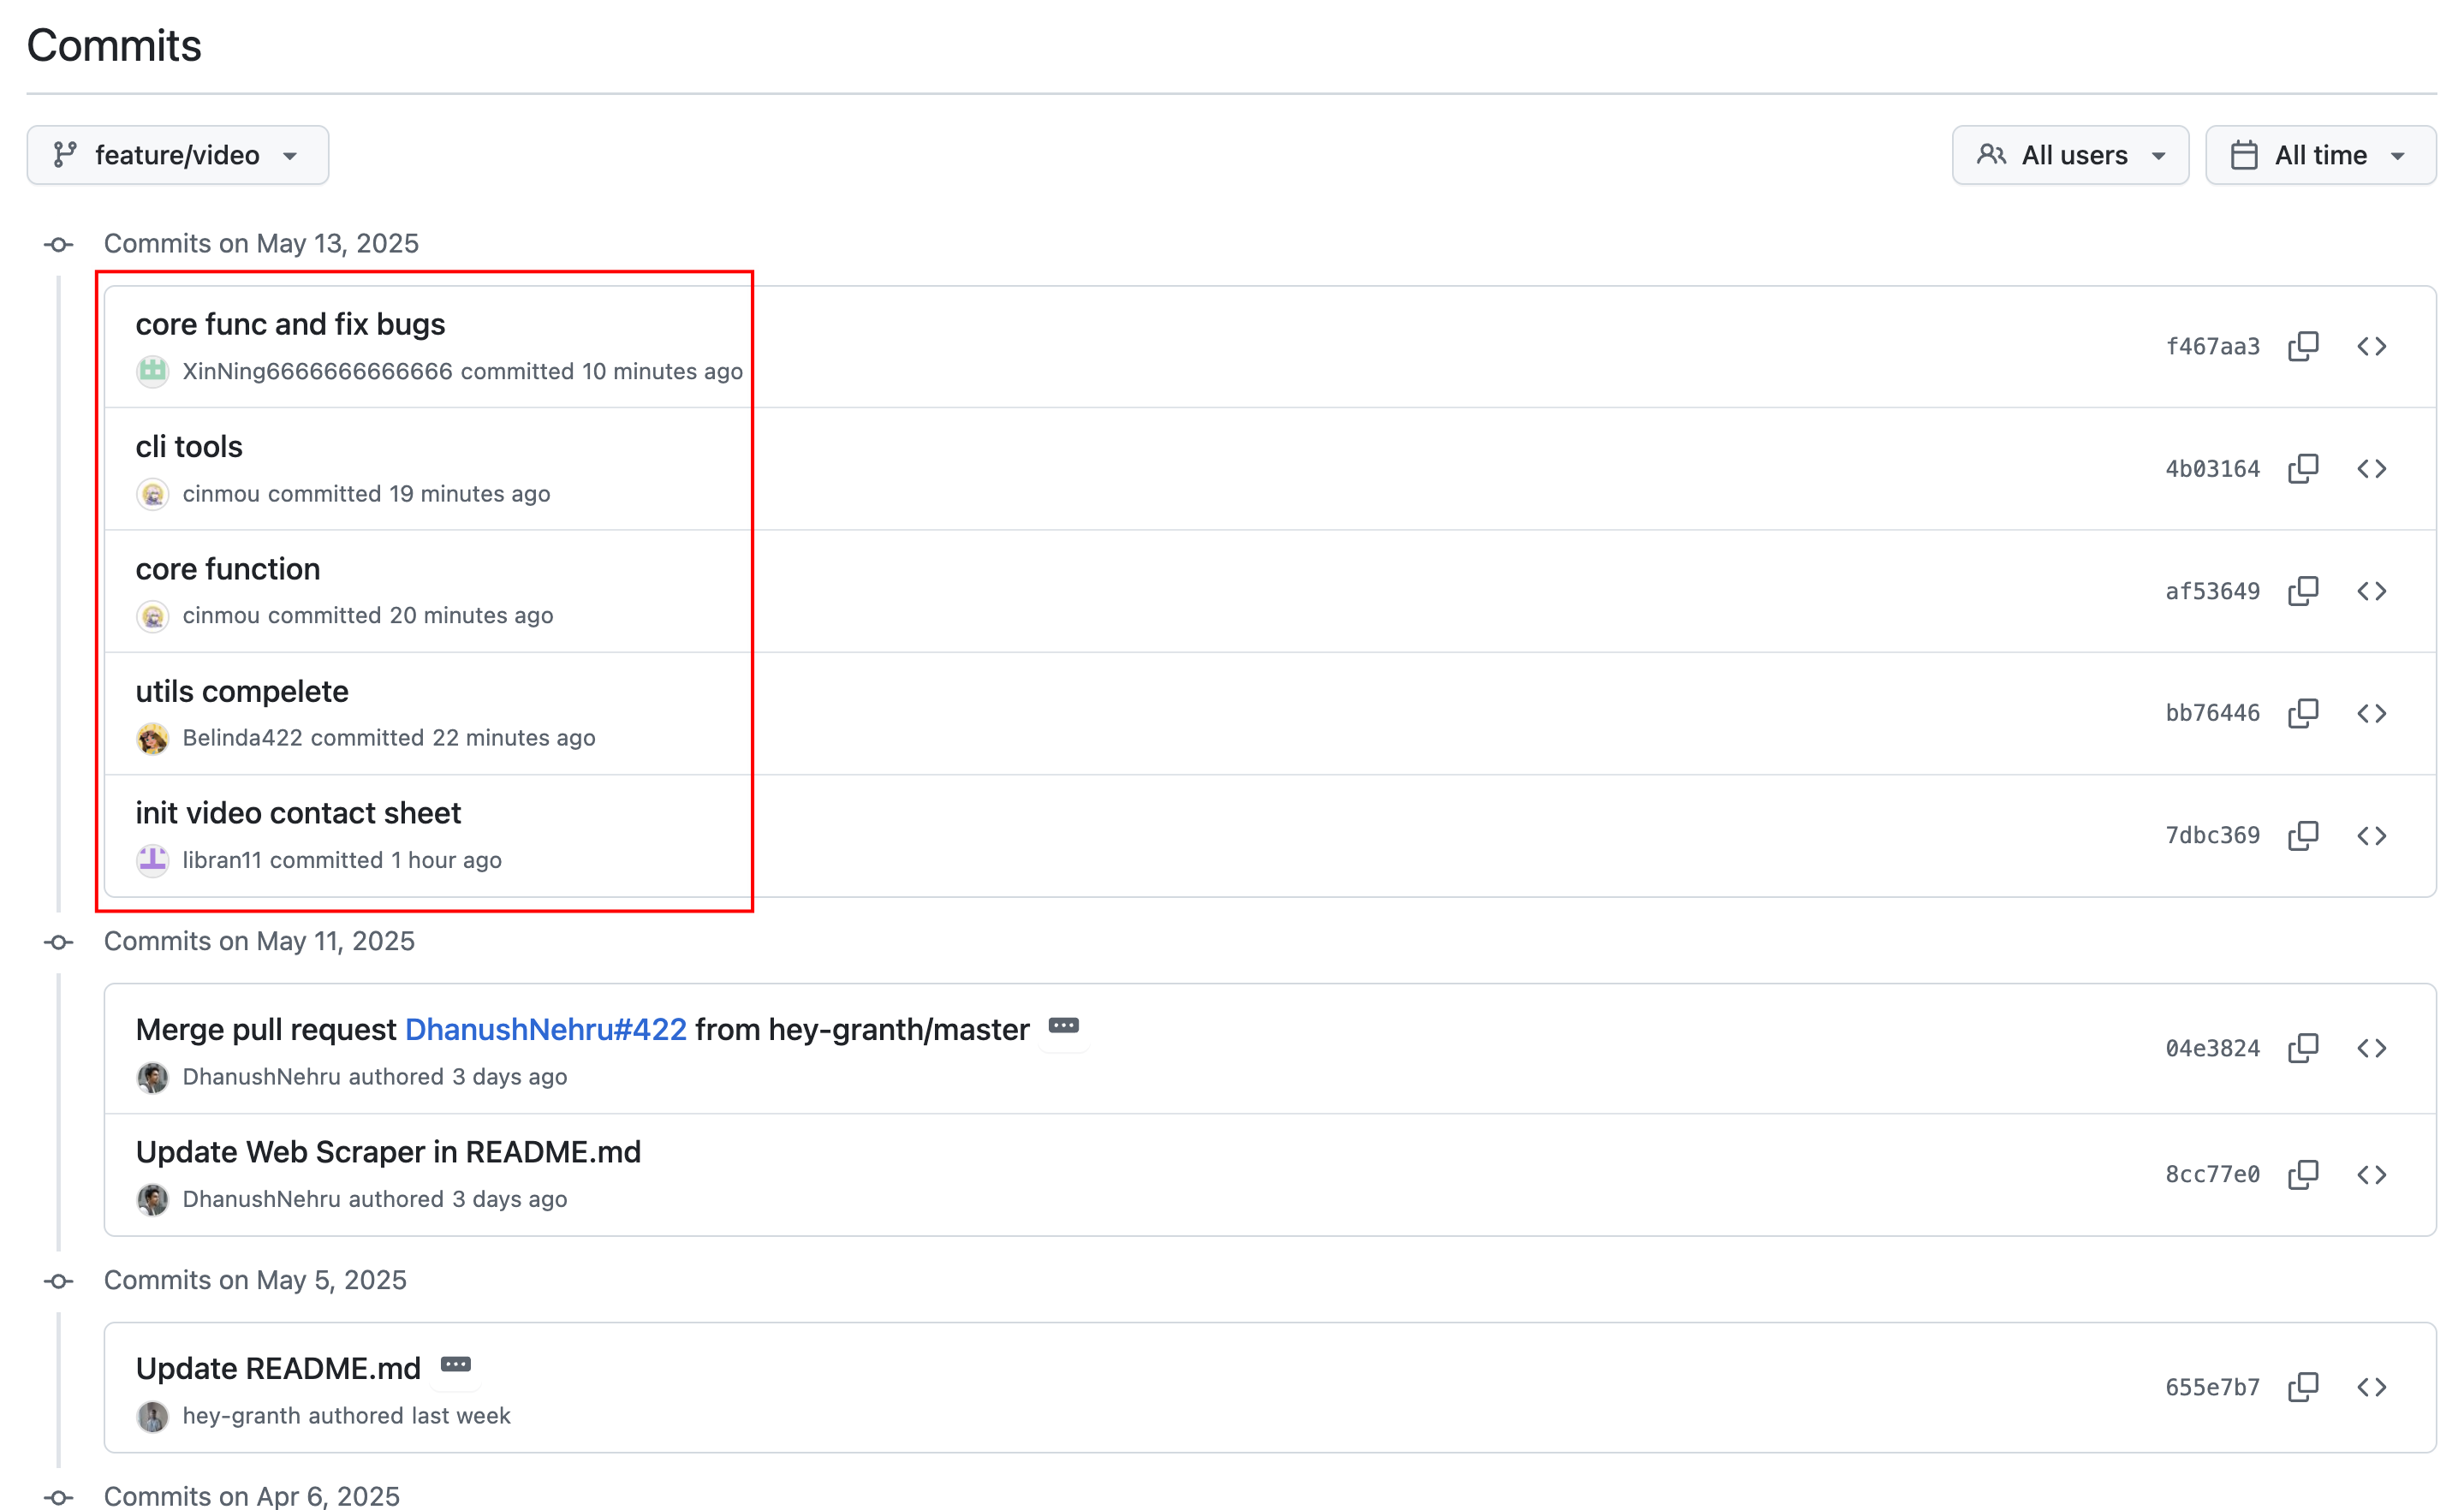
\includegraphics[width=\linewidth]{pic/commit.png}
    \caption{Relevant commit record}
    \label{fig:commit}
  \end{subfigure}
  \caption{Issue tracking and individual commit proof.}
\end{figure}

%--- Single image: pull request --------------------------
\begin{figure}[htbp]
  \centering
  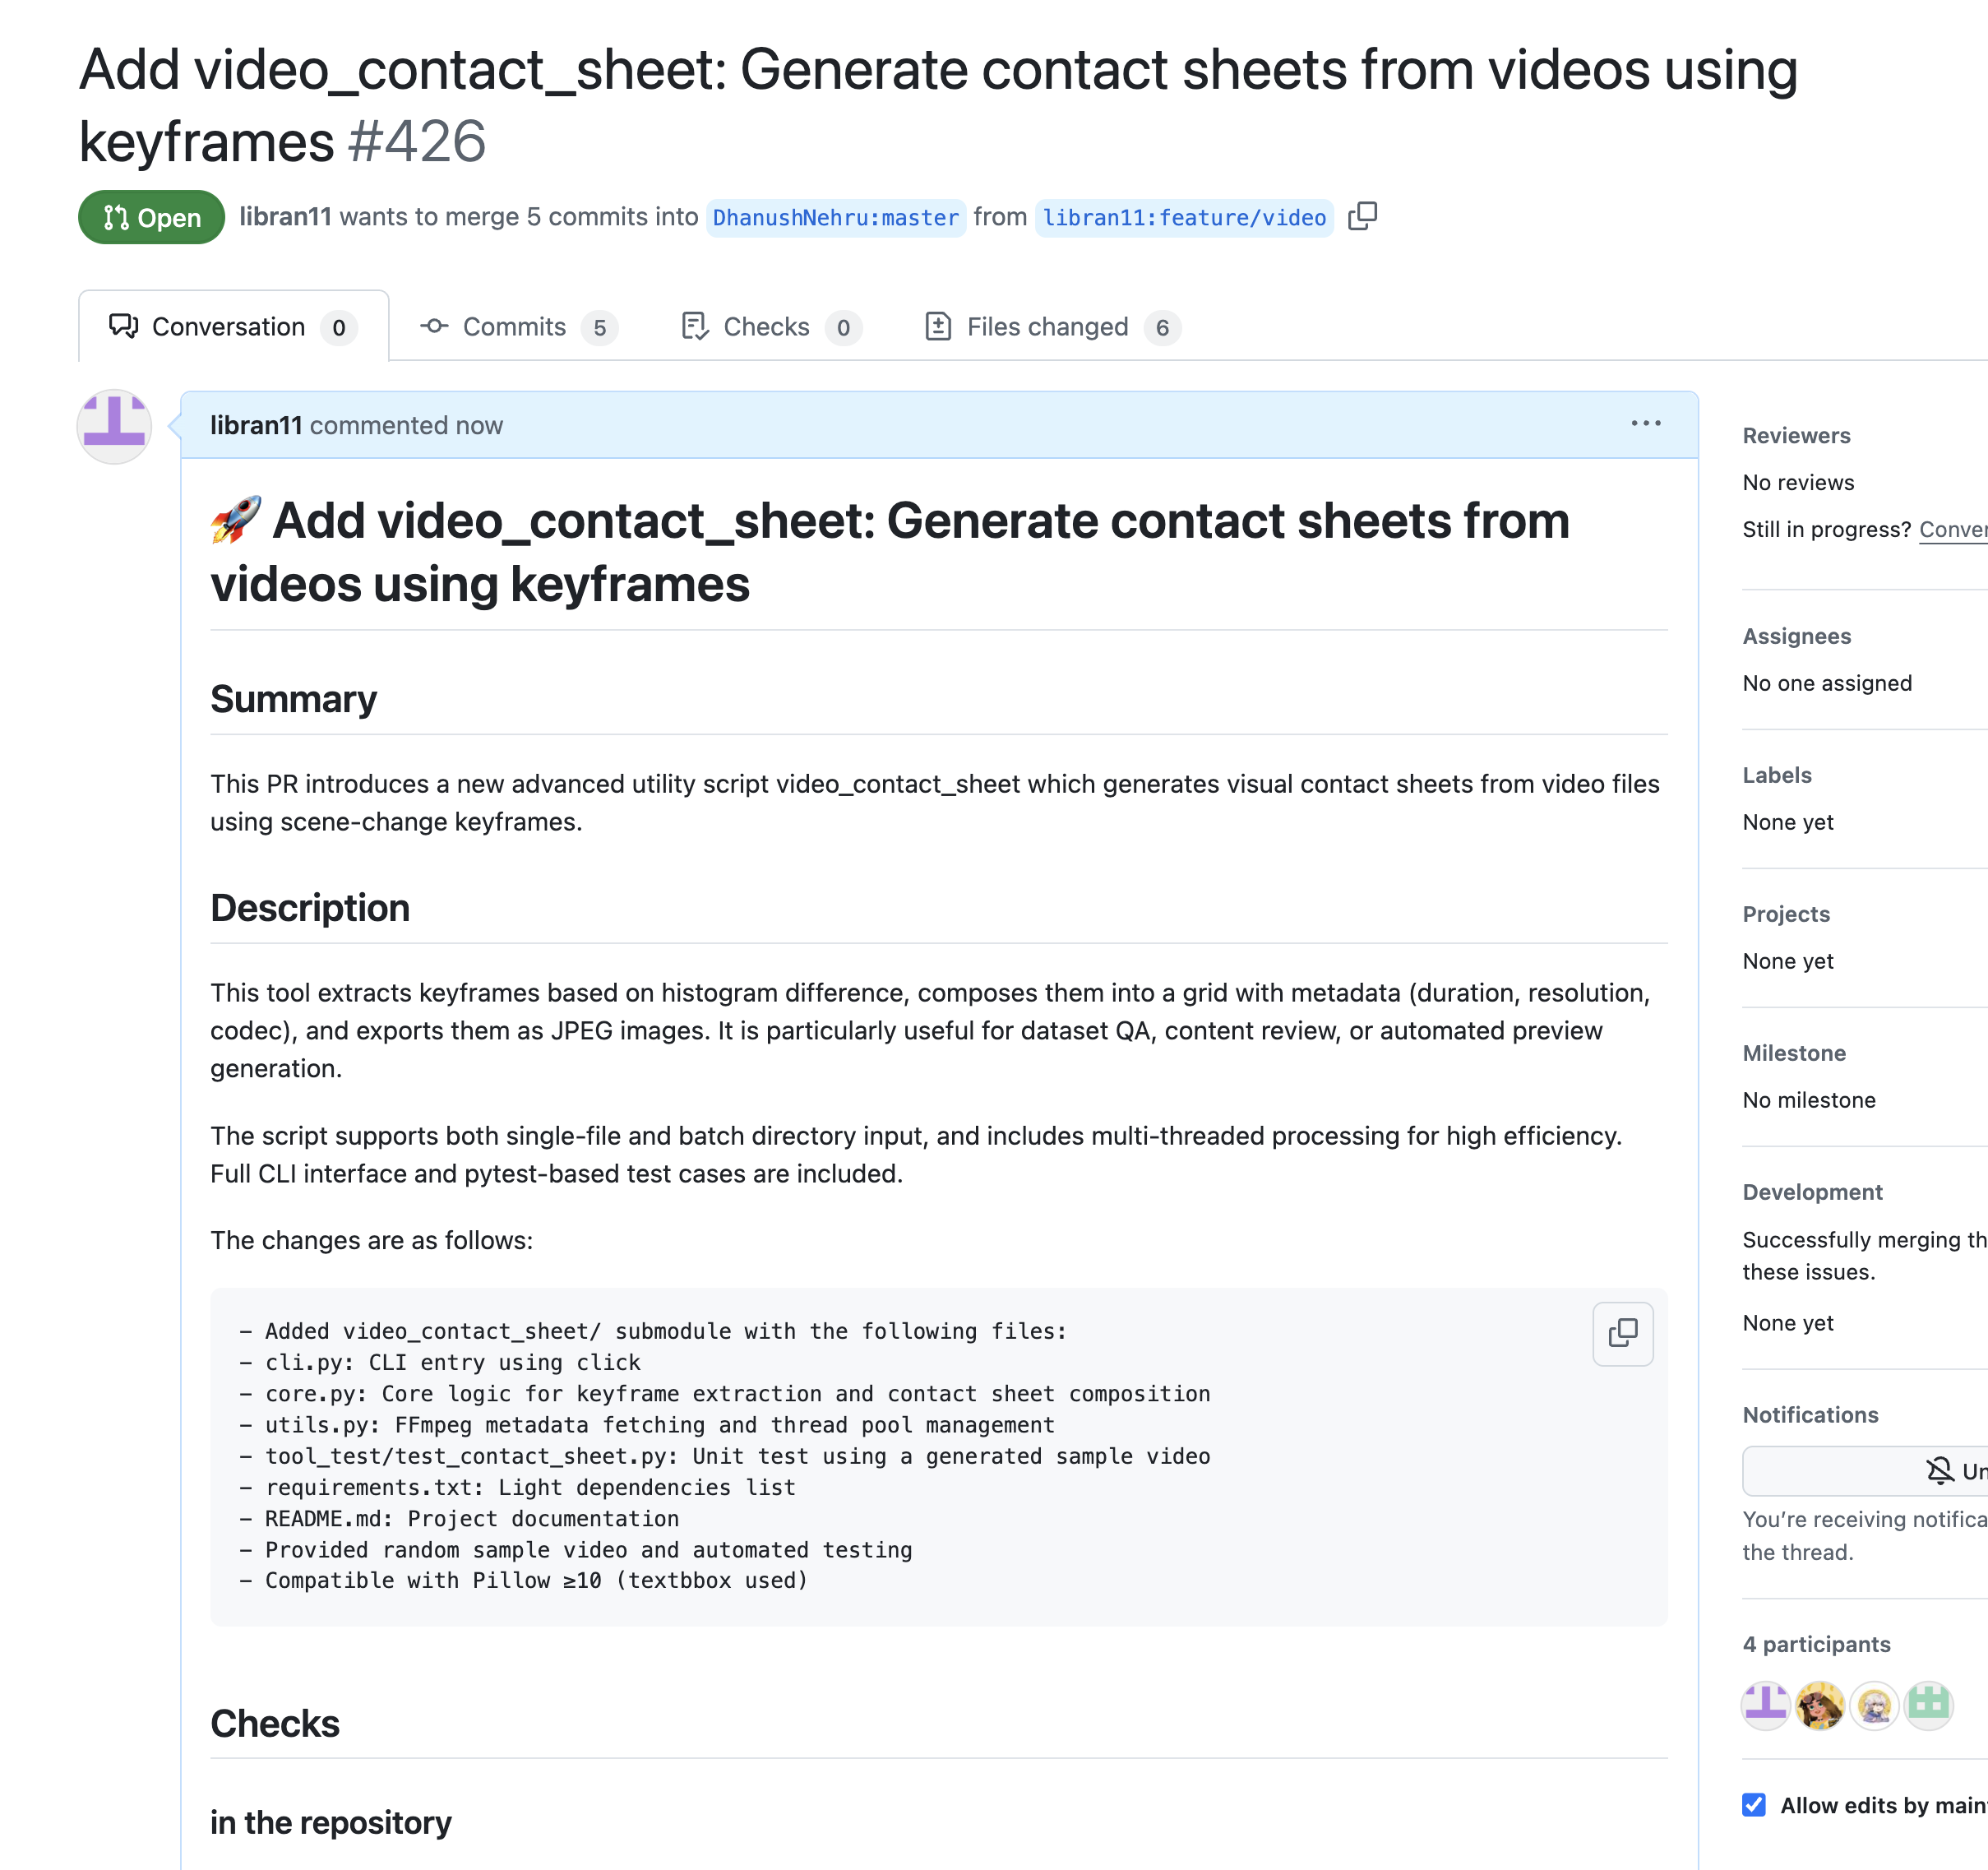
\includegraphics[width=0.50\textwidth]{pic/pullrequest.png}
  \caption{Final pull-request showing the integrated contribution.}
  \label{fig:pullrequest}
\end{figure}
%----------------------------------------


% ----------------------
% 6. Discussion
% ----------------------
\section{Discussion}
During this open-source contribution, our group participated in expanding the functionality of the Python-Scripts project on GitHub by submitting a new module, \textit{video\_contact\_sheet}, which extracts keyframes from videos and generates contact sheet images. We completed the full process from topic selection and design to coding, testing, and submitting a pull request, following standard open-source collaboration practices.

Throughout the contribution, we experienced the community’s strong focus on practicality and code maintainability. The maintainers provided clear issue and PR templates and emphasized coding standards. This process enhanced our skills in Git collaboration, coding conventions, and documentation, while deepening our understanding of how open-source projects operate.

% ----------------------
% 7. Conclusion
% ----------------------
\section{Conclusion}
In this project, our group first collaborated to complete a survey of open source contributions, including the significance of open source and how to become an open source contributor. Then we selected an actual meaningful open source project \texttt{Python-Scripts}, and actually contributed to the project. Through this course, we learned Git skills and the standard contribution process, and learned how to use git for team collaboration. We plan to continue to pay attention to open source projects outside of this course and continue to contribute.


% ----------------------
% References
% ----------------------
\section*{References}
\begin{itemize}
    \item \texttt{Python-Scripts} GitHub Repo: \url{https://github.com/DhanushNehru/Python-Scripts}
    \item GitHub Docs: \url{https://docs.github.com/}
    \item First Contributions Guide: \url{https://firstcontributions.github.io}
    \item Open Source Guides: \url{https://opensource.guide/}
\end{itemize}

% ----------------------
% Appendix
% ----------------------
\newpage
\appendix
\section*{Appendix}

\begin{center}
    \LARGE \textbf{CPT304 Assignment 2} \\
    \vspace{0.5em}
    \large \textbf{Individual Contribution}
\end{center}

\vspace{2em}

\noindent\textbf{Group Number:}

\vspace{1.5em}

\renewcommand{\arraystretch}{1.8}
\begin{tabular}{|>{\arraybackslash}m{5cm}|>{\centering\arraybackslash}m{4cm}|>{\centering\arraybackslash}m{3cm}|}
\hline
\textbf{Name} & \textbf{ID Number} & \textbf{Contribution (\%)} \\
\hline
1. &  &  \\
\hline
2. &  &  \\
\hline
3. &  &  \\
\hline
4. &  &  \\
\hline
\end{tabular}

\vspace{3em}

\noindent\textbf{Signed by all members:}

\vspace{1em}

\noindent\rule{16cm}{0.4pt}

\end{document}